% Formato para un capítulo cualquiera

%Título del capítulo
\chapter{Introducción.} 

\section{Qué es SNSAngelGuard}
SNSAngelGuard es una herramienta software diseñada en la Universidad de Alcalá en colaboración con otras universidades a nivel nacional con el objetivo de crear una aplicación que permita profundizar en el amplio universo de las redes sociales. Este proyecto forma parte de un proyecto global cuyo objetivo es desarrollar herramientas para simular el comportamiento de una Red Social, sea cual fuere su naturaleza, y comprender su comportamiento, por medio de modelado de datos y construcción de protocolos.En este proyecto se pretenden dos objetivos:

\begin{enumerate}
\item Construcción de un modelo de datos general para el conjunto de redes sociales existentes, haciendo un estudio de aquellas partes en las que dichas redes sociales pueden llegar a un punto en común en el almacenamiento de datos.
\item Diseñar y desarrollar una aplicación que extraiga datos de una determinada Red Social y que trate dichos datos con una funcionalidad determinada. En éste caso, la red social a tratar será Facebook.
\end{enumerate}


\section{Concepto de Red Social}
Como concepto, una Red Social puede entenderse como un ente formado por un conjunto de personas que comparten algún tipo de relación (familiares, amigos, trabajo, ocio..., etc.) o simplemente, por personas que quieren compartir su conocimiento para llevar a cabo un objetivo común. Dentro de una Red Social, cada persona puede comunicarse con las personas que forman su entorno, además de tener nuevas relaciones y darse a conocer dentro de otros entornos que a su vez, todos juntos, conformen dicha red.
\bigskip
\par
Las redes sociales tienen su origen en la teoría de los “Seis grados de separación”. Esta teoría se basa en la idea de que una persona puede estar conectada con cualquier otra persona del planeta a través de una cadena de no más de seis intermediarios. Dicho de otra forma, las redes sociales se basan en el simple hecho de que el número de conocidos crece exponencialmente con el número de enlaces de la cadena, y sólo un pequeño número de enlaces son necesarios para que el conjunto de conocidos se convierta en una población humana entera.
\bigskip
\par
Si ponemos ésta idea en práctica, podemos comprobar que no es nada descabellada. Cada persona se suele relacionar con aproximadamente unas 100 personas, entre familiares, amigos, compañeros de trabajo,..., etc. Si cada una de estas personas se relaciona con otras 100 personas no comunes, no es difícil imaginarse que una persona puede difundir un mensaje entre 10000 personas. Si seguimos recorriendo eslabones en la cadena de relaciones, en unos cuantos pasos estaríamos preparados para mandar un mensaje a cualquier persona que estuviera conectada a una Red Social. Dicho de otra manera, estaríamos preparados para
entrar en contacto con cualquier persona del planeta.
\bigskip
\par
El verdadero impacto que tiene una Red Social sobre la sociedad actual moderna no tiene límites. Nos encontramos ante un fenómeno de masas, con una capacidad de comunicación imposible de calcular. Por esta razón, el estudio de las Redes Sociales se ha
convertido en un elemento esencial para las Universidades y Centros de Conocimiento y, sin ir más lejos, para todas aquellas empresas, tanto grandes, medianas o pequeñas, que quieran expandirse y dar a conocer sus productos. Cualquier departamento de marketing incorpora especialistas en redes sociales para calcular el impacto de sus productos en la sociedad y difundirlos de la manera más eficaz posible.
\bigskip
\par
Evidentemente, todas estas relaciones serían imposibles sin un vehículo idóneo de comunicación. Gracias al desarrollo tecnológico del sector de la informática y de las telecomunicaciones, cualquier persona puede disponer de un equipo informático
moderadamente asequible y una conexión a Internet lo suficientemente rápida como para poder estar en constante comunicación con otra, y poder enviar y recibir mensajes simultáneamente, como si ésta comunicación se produjera “cara a cara”.
\section{OpenSocial}
OpenSocial es un conjunto de API comunes destinadas a la creación de aplicaciones sociales en múltiples sitios web. OpenSocial está compuesto por API de JavaScript y API de datos de Google. La existencia de este modelo de programación único resulta de gran utilidad tanto para los desarrolladores como para los sitios web. 
\bigskip
\par
En primer lugar, los desarrolladores sólo tienen que aprender las API una vez para crear aplicaciones que funcionen con cualquier sitio web compatible con OpenSocial. 
\bigskip
\par
En segundo lugar, como cualquier sitio web puede implementar OpenSocial, los desarrolladores disponen de una amplia red de distribución para llegar a los usuarios. Los sitios web también se benefician mediante la participación de un conjunto mucho más numeroso de desarrolladores externos que el que podrían conseguir sin un conjunto estándar de API. 
\bigskip
\par
La Compañía Google y sus asociados, ofrecen algunas tecnologías para que Internet en su conjunto llegue a ser un medio más social, respondiendo así al claro interés de los usuarios. Productos, como orkut, son sólo uno de los distintos sitios web que implementan OpenSocial. Actualmente, el código de ejemplo se ofrece con la licencia de Apache 2.0. Además, las licencias de toda la documentación de OpenSocial proceden de Creative Commons, por lo que se puede reutilizar y combinar los servicios como estimes oportuno. En el futuro, se plantea ofrecer el software libre de los componentes necesarios para ejecutar OpenSocial en tu propio sitio web.
\subsection{Estructura básica de una aplicación que utiliza el API de OpenSocial}
Las aplicaciones de OpenSocial utilizan la estructura de gadgets de Google, pero con extensiones que proporcionan acceso programático a datos sociales dentro de su entorno de contenedor. De forma similar a los gadgets de Google, las aplicaciones de OpenSocial alojan documentos XML con lenguaje HTML/JavaScript integrado. Las aplicaciones sociales disponen de la mayor parte de la infraestructura de los gadgets de Google, pero con algunas pequeñas excepciones. Uno de los primeros entornos de las aplicaciones sociales que utilizan las API de OpenSocial es orkut. Se espera que otros sitios web compatibles con OpenSocial admitan pronto la participación de desarrolladores.
\subsection{Crear aplicaciones con OpenSocial}
Las aplicaciones sociales se crean en principio de la misma forma que los gadgets de Google: con tu editor de texto favorito o con el Editor de gadgets de Google. A continuación, se pueden aumentar con las API JavaScript de OpenSocial, donde estas aplicaciones pueden obtener y enviar datos sociales sobre amigos y actividades.

\section{Facebook}
Facebook es el ejemplo de Red Social, mundialmente conocido. Facebook es una aplicación que engloba una conjunto de redes sociales creada por
Mark Zuckerberg. Se trata de una aplicación web en la cualquier usuario puede acceder a ella a través de únicamente una dirección de correo válida. En ella, el usuario puede ponerse en contacto con otros usuarios de una o más redes sociales, dependiendo de su situación académica, su lugar de trabajo o su región geográfica.
\bigskip
\par
Originalmente se creó específicamente para estudiantes de Harvard, Universidad en la que inició sus estudios su creador, pero posteriormente, tras su éxito a nivel mundial, fue ampliada a cualquier persona que tuviera una dirección de correo electrónico.
\bigskip
\par
Una de las características principales de Facebook es su expansión hacia el mundo de las aplicaciones web. Se ha convertido en una plataforma en la que terceros pueden desarrollar aplicaciones y hacer negocio a partir de la red social.
\bigskip
\par
Para conseguir dicho objetivo, el equipo de Facebook ha ido publicando diferentes APIs, basadas en Servicios Web, para la creación de aplicaciones y el acceso a datos de usuario, las cuales van adaptándose a las tecnologías actuales y marcando un perfil de aplicación determinado. Cualquier desarrollador tiene acceso a ellas y constituyen una de las mayores riquezas actuales de la compañía.
\bigskip
\par
Actualmente, un desarrollador puede empezar una aplicación enfocándola directamente sobre el tipo de dispositivo para el que va dirigido. Las interfaces
publicadas por Facebook así lo establecen, dejando a la elección del programador el tipo de aplicación que desea realizar, tales como páginas web, aplicaciones para dispositivos móviles o aplicaciones para escritorio.
\subsection{Tipos de APIs}
Actualmente, Facebook dispone de las siguientes interfaces para el desarrollo de
aplicaciones:
\begin{enumerate}
\item Login: Es una interfaz que integra los métodos de logueo necesarios para una aplicación web. Puede ser utilizada desde cualquier lenguaje de programación pero es excesivamente sencillo de utilizar en el lenguaje JavaScript.
\item GraphApi: Es la interfaz más utilizada y más universal. Permite acceder a los datos de un usuario por medio de objetos o entidades que pueden ser tratadas posteriormente a través de la aplicación.
\item FQL: Son las siglas de Facebook Query Language o, dicho de otra manera, es el lenguaje de SQL de Facebook para el acceso a datos de usuario.
\item Legacy REST API: Es el conjunto de servicios REST que Facebook puso en
disposición para el acceso a datos mediante peticiones HTTP. Es el más antiguo de
todos y está próximo a la desaparición.
\end{enumerate} 

\subsection{RestFB}
En la actualidad, el creciente volumen de desarrolladores que trabajan en proyectos de aplicaciones de Facebook ha desencadenado una oleada de apariciones de arquitecturas o proyectos que encapsulan el acceso a las interfaces ofrecidas por Facebook y hacen más fácil trabajar con esta. Con estas nuevas arquitecturas, se ofrece el acceso a toda la funcionalidad de Facebook mediante clases de cualquier lenguaje de programación. RestFB es una de estas arquitecturas.
\bigskip
\par
RestFB engloba las APIs de Facebook Grap API y Old REST API mediante un cliente escrito en el lenguaje de programación JAVA. Tiene las siguientes características:
\begin{enumerate}
\item Es totalmente transparente a la interfaz que se utiliza para el acceso a datos de Facebook. El programador no conoce con certeza qué interfaz se está utilizando.
\item Su api es mínima, ya que engloba una serie de métodos públicos que son configurables utilizando las sentencias FQL proporcionadas por Facebook, por lo que los métodos definidos en sus interfaces son realmente pocos.
\item Los cambios que se pueden producir por parte de Facebook en su interfaz son automáticamente absorbidos, haciendo que el usuario no cambie su forma de
desarrollar la aplicación.
\item Para configurarlo, no hay más que introducir su dependencia Maven correspondiente en el pom.xml del proyecto.
\item No guarda dependencias con ningún otro módulo.
\item El transporte de datos se realiza mediante lenguaje XML o JSON, pudiendo ser parseado al llegar a la aplicación dependiendo de las necesidades funcionales del módulo.
\end{enumerate} 
Por todas estas razones, esta arquitectura ha sido la elegida para llevar a cabo las interacciones con Facebook desde SNSAngelGuard.

\section{Servicios Web}
\subsection{¿Qué es un Servicio Web?}
El consorcio W3C\footnote[1]{World Wide Web Consortium: Comunidad internacional que desarrolla estándares que aseguran el crecimiento de la Web a largo plazo. Fuente www.w3c.es} define a los Servicios Web como sistemas software diseñados para soportar una interacción interoperable maquina a máquina sobre la red. Dichos servicios suelen ser presentados en forma de APIs Web que pueden ser accedidas en una red (principalmente Internet) por medio de una aplicación y se suelen ejecutar en la máquina que los aloja.
\bigskip
\par
Hay muchas definiciones para éstos servicios pero la idea general se refiere a clientes  y servidores que se comunican entre sí mediante mensajes XML\footnote[2]{Son las siglas de Extensible Markup Language, una especificación/lenguaje de programación desarrollada por W3C. XML es una versión de SGML, diseñado especialmente para documentos de la red. Permite que los desarrolladores creen sus propias etiquetas, permitiendo la definición, transmisión, validación e interpretación de datos entre aplicaciones y entre organizaciones.} los cuales siguen el estándar SOAP\footnote[3]{Son las siglas de Simple Object Access Protocol. Protocolo estándar que define cómo dos objetos en diferentes procesos pueden comunicarse por medio de intercambio de datos XML.}.
\bigskip
\par
En estos últimos años, se ha popularizado una arquitectura de Servicio Web denominada REST\footnote[4]{Son las siglas de Representational State Transfer.}. Esta arquitectura se ha convertido en una nueva opción para decantarse por tecnología basada en Servicios Web. En éste caso, tenemos tres opciones:
\begin{enumerate}
\item Llamadas a Procedimientos Remotos (RPC, Remote Procedure Call): Estos servicios presentan una interfaz de llamada a procedimientos y funciones distribuidas, lo cual es muy familiar a la mayoría de los desarrolladores. Normalmente, la unidad básica de uso de éste servicio es la operación WSDL\footnote[5]{Son las siglas de Web Service Description Language, un formato XML que se utiliza para describir Servicios Web. Describe la interfaz pública de un Servicio Web. Está basado en XML y describe la forma de comunicación, es decir, los requisitos del protocolo y los formatos de mensaje necesarios para interactuar con los servicios listados en su catálogo. Las operaciones y mensajes que soporta se describen en abstracto y se ligan después al protocolo concreto de red y al formato del mensaje.}.
\bigskip
\par
Las primeras herramientas para Servicios Web estaban centradas en éste tipo de enfoque, es por esta razón que son denominados Servicios Web de primera generación y su uso está muy extendido. Sin embargo, ha sido ampliamente criticado y muchos expertos creen que debería desaparecer, ya que su implementación se basa en el mapeo de servicios directamente a funciones específicas del lenguaje o llamadas a métodos.
\item Arquitectura Orientada a Servicios SOA\footnote[6]{Son las siglas de Service Oriented Architecture.}: Según la arquitectura de llamadas a Procedimientos Remotos, la unidad básica de operación es la Operación. En el caso de los Servicios SOA, se trata de implementar Servicios Web a través del mensaje, que en éste caso será la unidad básica de operación. Esta arquitectura también es conocida como Servicio Orientado a Mensajes.
\item Servicios REST: Son Servicios Web que intentan basarse en protocolos HTTP o similares. Su objetivo es restringir el uso de una interfaz a un conjunto de operaciones estándar universalmente conocidas (GET, PUT, POST, DELETE). Por lo tanto, esta arquitectura se basa en interactuar con recursos con estado en vez de mensajes u operaciones. 
\end{enumerate}
\subsection{Arquitectura REST}
\subsubsection{Introducción}
REST es un estilo de arquitectura Software diseñado para el intercambio de datos en sistemas distribuidos. Fue introducido en la tesis doctoral de Roy Fielding en el año 2000, el cual es uno de los principales autores de la especificación HTTP.
\bigskip
\par
Los servicios REST se basan en el concepto  de “Todo recurso  (información) debe tener y ser accesible mediante una URI única”. A partir de éste concepto, se usan los métodos de comunicación web sobre HTTP (GET, PUT, POST, DELETE)  para definir diferentes acciones predefinidas sobre los recursos “URIs”.
Las características básicas de los servicios REST son los siguientes:
\begin{enumerate}
\item Todo recurso debe tener una URI única.
\item Los recursos son enlazados entre sí.
\item Uso de tecnología estándar (HTTP, XML, JSON,…, etc).
\item El recurso puede tener múltiples representaciones dependiendo de la solicitud.	
\end{enumerate}
La figura 1.1 representa la arquitectura de la tecnología REST:
\begin{figure}
\begin{center}
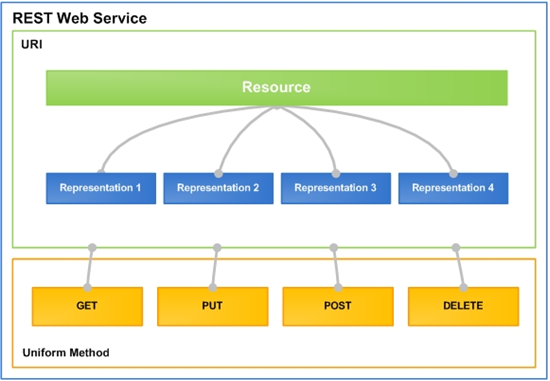
\includegraphics[width=12cm,height=8cm]{Figuras/REST.png}
\end{center}
\caption{\label{REST} Arquitectura de la tecnología REST}
\end{figure}
\subsubsection{Principios básicos}
\begin{enumerate}
\item Escalabilidad de la interacción con los componentes: Un determinado sitio web puede crecer exponencialmente sin degradar su rendimiento. Varios sistemas pueden acceder y utilizar servicios REST simultáneamente sin que esto degrade el rendimiento de la aplicación.
\item Interfaces estándar: Gracias al protocolo HTTP, cualquier cliente puede interactuar con un servicio REST sin necesidad de una configuración especial, únicamente definiendo la URI característica del propio recurso
\item Funcionamiento independiente de la arquitectura: Al ser una arquitectura basada en protocolos HTTP y estándares de intercambio de mensajes, permite adaptarse a cualquier tipo de cliente, ya que HTTP permite la extensibilidad mediante el uso de cabeceras a través de las URIs.
\item Es compatible con sistemas intermedios: Pueden ser utilizados en combinación con proxys para Web, herramientas de mejora de la seguridad, como firewalls y con herramientas de encapsulado para la Web, como es el caso de los gateways.  
\end{enumerate}
\bigskip
\par
REST logra conseguir estos objetivos aplicando las siguientes restricciones:
\begin{enumerate}
\item Identificación de recursos y manipulación de ellos a través de representaciones. Esto se consigue a partir de URIs. HTTP es un protocolo centrado en URIs. Los recursos son objetos lógicos que intercambian mensajes con las entidades que requieran sus servicios. No pueden ser directamente accedidos o modificados, más bien se trabaja con representaciones de ellos, es decir, cuando invocamos al método PUT para modificar los datos de un recurso, realmente estamos enviándole como mensaje una representación de lo que debería ser. Internamente, el recurso es totalmente transparente, es decir, puede desde un registro de una entidad de base de datos, un fichero plano…
\bigskip
\par
\item Mensajes autodescriptivos. REST establece que los mensajes HTTP deben ser tan descriptivos como sea posible. Esto hace que los intermediarios interpreten los mensajes y ejecuten los servicios en nombre del usuario. HTTP logra este objetivo por medio de una definición de un método estándar (GET, PUT, POST, DELETE), muchas cabeceras y un método de direccionamiento. Por ejemplo, las cachés Web saben que, por defecto, el método GET es cacheable, sin embargo, el método POST no lo es. Además, saben cómo interpretar la información contenida en las cabeceras, es por esta razón por la cual, cuando una aplicación accede a un recurso de una base de datos por medio de un servicio REST, el navegador es capaz de obtener el usuario el cual intenta acceder y modificar dicha base de datos por medio de su cabecera.
\bigskip
\par
\item Hipermedia como mecanismo de estado de la aplicación. El estado actual de una aplicación web es capturado mediante archivos de hipertexto que son alojados tanto en el cliente como en el servidor de la aplicación. El servidor conoce en todo momento el estado de los recursos pero no intenta seguir la pista a las sesiones individuales de cada cliente. Este trabajo es realizado por el navegador, quien sabe navegar de recurso en recurso, recogiendo la información que él necesita para cambiar de un estado a otro dependiendo del servicio REST que esté ejecutando en cada momento.
\end{enumerate}
\subsection{Funcionalidad}
La funcionalidad básica de un servicio web se encuentra en el diseño de una interfaz que defina los métodos de acceso a los recursos para el resto de aplicaciones desde el servidor de la aplicación. Tras el diseño, esta interfaz se hará pública y las aplicaciones  podrán hacer uso de todos sus recursos aplicando las restricciones que se han planteado anteriormente. 
Esta es precisamente, la arquitectura que se ha definido para SNSAngelGuard y que se procederá a describir en los capítulos posteriores.